\documentclass[UTF8]{article}
\usepackage{geometry}
\usepackage{amsmath}
\usepackage{amssymb}
\usepackage{listings}
\usepackage{xcolor}
\usepackage{graphicx}
\usepackage{float}
\usepackage{subfigure}
\usepackage[amssymb]{SIunits}
\usepackage{cite}
\usepackage{hyperref}
\usepackage{matlab-prettifier}

\geometry{a4paper,scale=0.72}
\setlength{\parindent}{0pt}

% Renew some basic command
\newcommand{\ds}{\displaystyle}
\newcommand{\dx}{\mathrm{d}x}
\newcommand{\dy}{\mathrm{d}y}
\newcommand{\ul}{\underline}

% Set indent
\setlength{\parindent}{1em}
\setlength{\parskip}{1.5ex}

\lstset{
    flexiblecolumns,
    numbers = left,
    style=Matlab-bw
}

\title{\bf DoA Estimation}
\author{Zike,Xu \ Zhiyi,Wang \ Dinghao,Cheng}
\date{\today}
\begin{document}
\maketitle
% Make 
\tableofcontents

\newpage
% \begin{abstract}
% \centering \small {{context}}
% \end{abstract}

\section{Narrowband Estimation}
\hspace{0.5em} We have obtained a stimulation data with $J = 4$ sensors in \emph{Observations\_nb.mat}, and we want to estimate angles of the source with MUSIC algorithm.

In MUSIC, there're some basic arguments, $J$ represents the number of sensors, and $P$ represents the number of sources ($P < J$).
The signal is given in the form of
\begin{equation}
    s(t) = A(t)e^{j\omega_c t + \phi(t)}
\end{equation}
when $A(t)$ is the envelop, $\phi(t)$ is the phase. In narrowband, they varies slow than $e^{j \omega_c t}$,
\begin{gather}
    s(t - \tau) = A(t - \tau) e^{j\omega_c(t - \tau)}e^{j\phi(t - \tau)} \approx A(t)e^{j\omega_c(t - \tau) \phi(t)} = e^{-j\omega_c\tau}\cdot s(t)
\end{gather}
thus, in narrowband, Time delay $\approx$ Phase shift.

Position J sensors on x-y axis, their relative position can be $p_i = (x, y)^t$. Consider just one far field signal passes the system with angle $\theta$(with y axis), which can be expressed as $\ul{v} = (\sin \theta, \cos \theta)^t$. The time delay of every sensors is $p v$. Convert it into phase shift, its $e^{-j 2 \pi \omega_c \Delta t}$, denote it as $a(\omega, \theta)$. Thus, we can construct a matrix with $a(\omega, \theta)$ which can shift the original signal as $\theta$ changes.
\begin{gather}
    s[k, \ul{p_i}] = s[k] \cdot e^{j \omega \tau_i} = s[k] \cdot a_i(\omega, \theta)
\end{gather}
For narrowband signal, we can acquire its $f_c$(center frequency) in advance, so $a_i(\omega, \theta)$ can be written as $a_i(\theta)$.

We model the system as
\begin{gather*}
    \ul{x}[k] = (x_1[k], x_2[k], x_3[k], \cdots, x_J[k])^t \\
    \ul{n}[k] = (n_1[k], n_2[k], n_3[k], \cdots, n_J[k])^t \\
    \ul{a}(\theta) = (a_1(\theta), a_2(\theta), a_3(\theta), \cdots, a_J(\theta))^t
\end{gather*}
in which 
\begin{gather}
    \ul{x}[k] = \ul{a}(\theta) s[k] + \ul{n}[k]
\end{gather}
for multiple sound sources, add them together to get
\begin{gather}
    x_i[k] = \sum_{p}a_i(\theta_p) s_p[k] + n_i[k] \Rightarrow \ul{x}[k] = A \ul{s}[k] + \ul{n}[k]
\end{gather}
A is a $J \times P$ matrix, and $\ul{s}[k]$ is the column vector consists of different sound sources.

Denoted the covariance matrix as $R_x$, 
\begin{gather}
   R_x = \mathbb{E}\{\ul{x}[k]\ul{x}^h[k]\} 
\end{gather}
expand it with $\ul{x}[k] = A \ul{s}[k] + \ul{n}[k]$, 
\begin{gather}
    \mathbb{E}\{\ul{x}[k]\ul{x}^h[k]\} = \mathbb{E} \{ (A \ul{s}[k] + \ul{n}[k])(A \ul{s}[k] + \ul{n}[k])^h \} \Rightarrow A \mathbb{E}\{ \ul{s}[k]\ul{s}^h[k] \}A^h + \mathbb{E}\{ \ul{n}[k] \ul{n}^h[k]\}
\end{gather}
$R_s = \mathbb{E}\{ \ul{s}[k]\ul{s}^h[k] \}$ is a Hermite positive definite matrix, so 
\begin{gather*}
   \mathrm{rank}(R_s) = \mathrm{rank}(A) = \mathrm{rank}(A R_s A^h) = P_{source}
\end{gather*}
The rank of the matrix equals to its number of non-zero eigenvalues, so $A R_s A^h$ contains $J - P$ zero eigenvalues. 

Let $\ul{u_i}$ be the eigenvector corresponding to zero eigenvalues, so 
\begin{gather}
    \ul{u}_i^h A R_s A^h \ul{u}_i = \ul{0} \Rightarrow (A^h\ul{u}_i)^h R_s (A^h \ul{u}_i) = \ul{0} \Rightarrow A^h\ul{u}_i = \ul{0}
\end{gather}
Which claim that the $J - P$ zero eigenvectors is orthogonal to those steering vectors.

We traverse $\theta$ to get the minimal $\sum_{i}\ul{a}^h(\theta_p)\ul{u}_i$, and define
\begin{gather}
    P_{music}(\theta) = \dfrac{1}{\sum_{i = 1}^{J - P}\big|\ul{a}^h(\theta_p)\ul{u}_i \big|^2}
\end{gather}
and the maximum point is the direction of arrival(DoA).

\subsection{Find $f_c$ through frequency domain}

% Plot the figure
\begin{figure}[h]
    \centering
    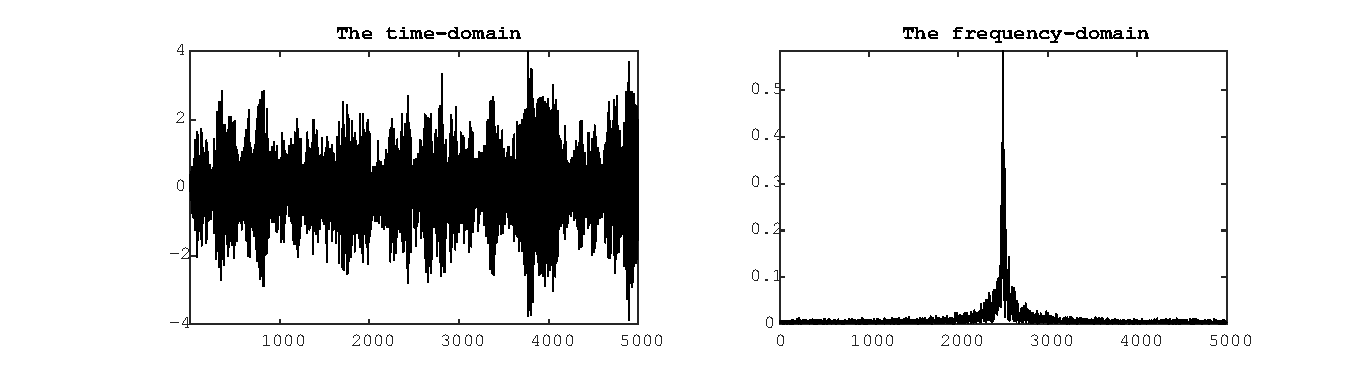
\includegraphics[scale=0.66]{img/fig02.eps}\\
\end{figure}

We can figure out from the graph that $f_c = 2500\hertz$.

\subsection{Estimate the DoA}
The MUSIC algorithm is implemented through MATLAB:
\lstinputlisting[
    style=Matlab-bw,
    caption = {\bf narrowband.m},
    label = {../src/narrowband.m}
]{../src/narrowband.m}

The result of the algorithm is:

\begin{figure}[H]
    \centering 
    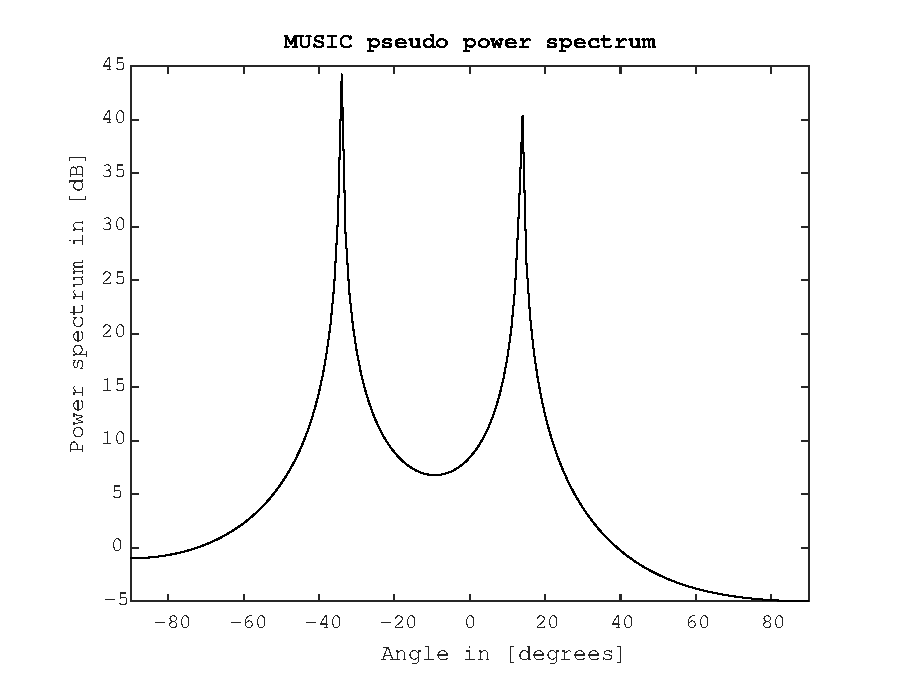
\includegraphics[scale=0.46]{img/fig01.eps}\\
\end{figure}

Which claims that:
\begin{lstlisting}
    The four microphones are ready !
    The desired source DOA with MUSIC is: -34 deg
    The interfering DOA with MUSIC is: 14 deg
\end{lstlisting}

\section{Broadband Estimation}
\hspace{0.5em} Since broadband speech signal can be non-stationary, we need STFT(Short-time Fourier Transform) to keep information on frequency domain and time domain at the same time.

The ISSM(Incoherent Signal Subspace Method), which perform STFT on the original signal, and do MUSIC with its result in row. We've read the original paper of ISSM, and ... Whatever, here I'm going to prove the map between frequency and the index in FFT.

In MATLAB, function FFT will perform
\begin{gather}
    Y[k] = \sum_{j = 1}^{n}{X[j]}e^{-i 2\pi(j - 1)(k - 1)/n}
\end{gather}

Thus, in case that the original signal $X[j] = e^{i 2 \pi f \cdot (j - 1) / f_s}$, 
\begin{gather*}
    Y[k] = \sum_{j = 1}^{n}{e^{i 2 \pi (j - 1)\big[\frac{f}{f_s} - \frac{k - 1}{n}\big]}}
\end{gather*}
The modulus of the result can reach its peak when k equals to some number. Let $u = \frac{f}{f_s} - \frac{k - 1}{n}$, using Euler's formula to transform it into $(u \neq 0)$
\begin{gather*}
    \mathrm{Re}\{ Y[k] \} = \sum_{j = 1}^n{\cos[ 2 \pi u \cdot (j - 1)]} = \frac{1}{2}(\csc(\pi \cdot u) \sin[(2n - 1)\pi \cdot u] + 1) \\
\mathrm{Im}\{ Y[k] \} = \sum_{j = 1}^n{\sin[ 2 \pi u \cdot (j - 1)]} = \frac{1}{2}\csc(\pi \cdot u)(\cos(\pi \cdot u) - \cos[(2n - 1)\pi \cdot u])
\end{gather*}
Consider the graph of $\csc$ function, and other $\sin$ or $\cos$ part limit it with an approximated 1 value, when u approach to 0, the modulus grows up quickly. And when $u = 0$, as $Y[k] = n$
\begin{gather}
    \frac{f}{f_s} = \frac{k - 1}{n} \Rightarrow f = \frac{(k - 1)f_s}{n}
\end{gather}

\subsection{Plot the wave and frequency response}
The figure:
\begin{figure}[H]
    \centering 
    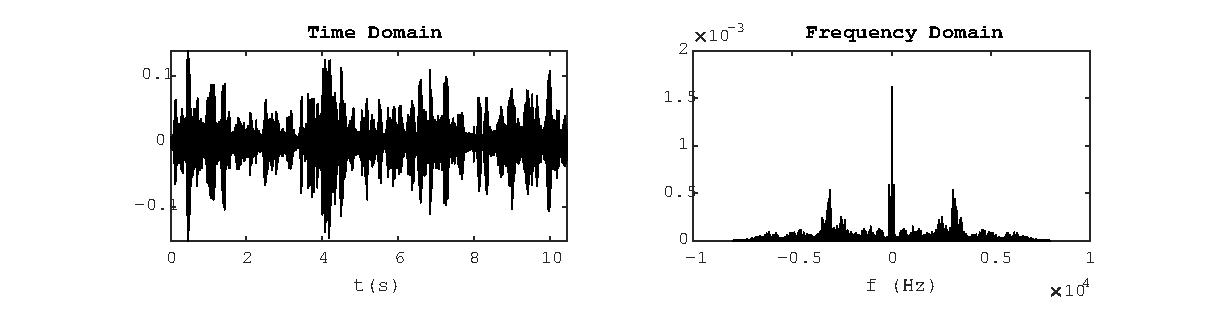
\includegraphics[scale=0.7]{img/fig03.eps}\\
\end{figure}
Its easy to figure out that the frequency covers a wide span of frequency and can not find a $f_c$.

\subsection{Perform STFT and MUSIC with spectral density matrix}
\hspace{0.5em} The processes of ISSM are
\begin{enumerate}
    \item Perform STFT on the original signal matrix.
    \item Perform MUSIC with some of its frequency span.
    \item Add them together, get the result.
\end{enumerate}

The ISSM algorithm is implemented through MATLAB:

\lstinputlisting[
    style = Matlab-bw,
    caption = {\bf broadband.m},
    label = {../src/broadband.m}
]{../src/broadband.m}

The result of the algorithm is(STFT Para: [len = 512/inc = 512]):

\begin{figure}[H]
    \centering
    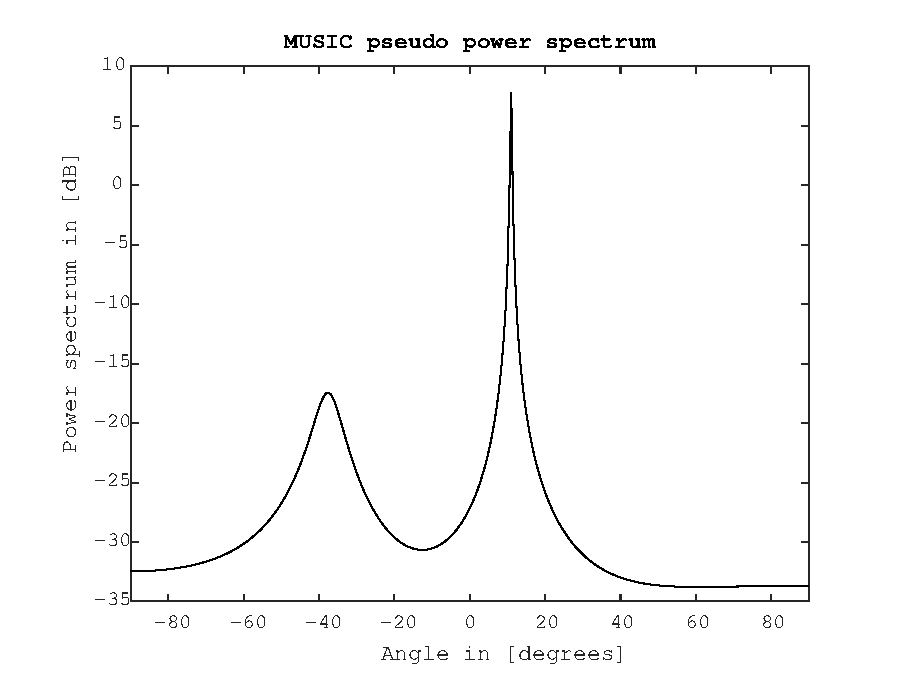
\includegraphics[scale=0.5]{img/fig04.eps} \\
\end{figure}

Which claims that:
\begin{lstlisting}
    The first source with MUSIC is: 38 deg
    The second source with MUSIC is: -11 deg
\end{lstlisting}

\section{Microphone Array Experiment(with bonus)}
\subsection{Adjustment}
\hspace{0.5em} Real time circumstance is rather complex than the stimulation data, so there's more special cases to deal with. For example, if the result have a long vacant span, there will be a high peak in $deg = 0$ which will interfer our result.

There're multiple solutions to the problem, we can fillter the low frequency band $[0, 20]$ to mitigate the impact of vacant span. Or we can filter the result with its power spectrum. In a word, there's ways through time domain and frequency domain to solve the problem. We chose the former method.

And we apply window function to reduce error. Apply the hanning window function to the segments of STFT, $x[s:e]H^t$ to get the signal.

Here are the figures before and after the optimization:
\begin{figure}[H]
    \centering
    \subfigure[before window]{
        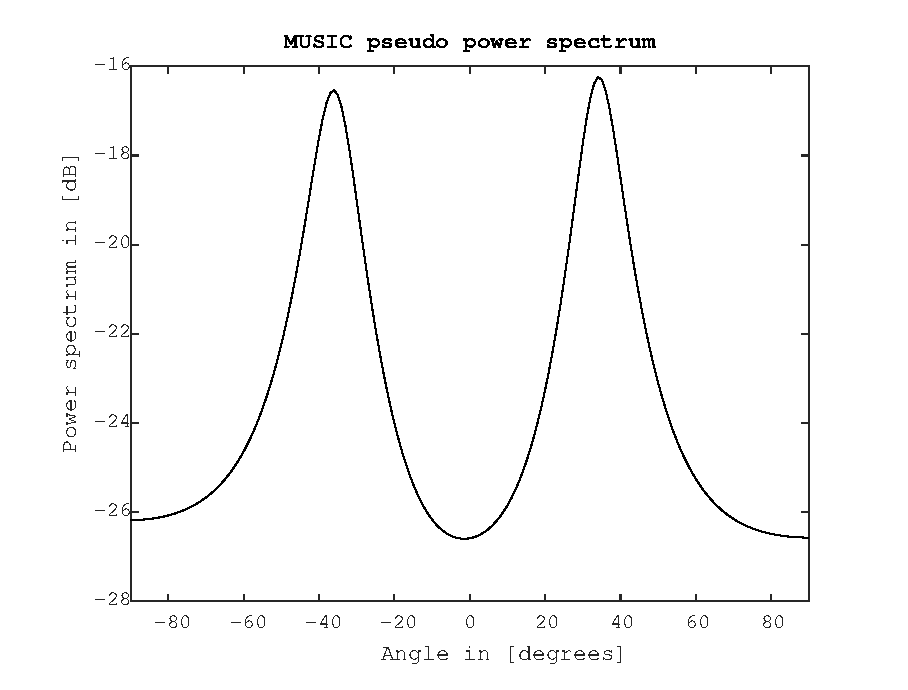
\includegraphics[scale=0.4]{img/before_window.eps}}
    \hspace{0.4in}
    \subfigure[after window]{
        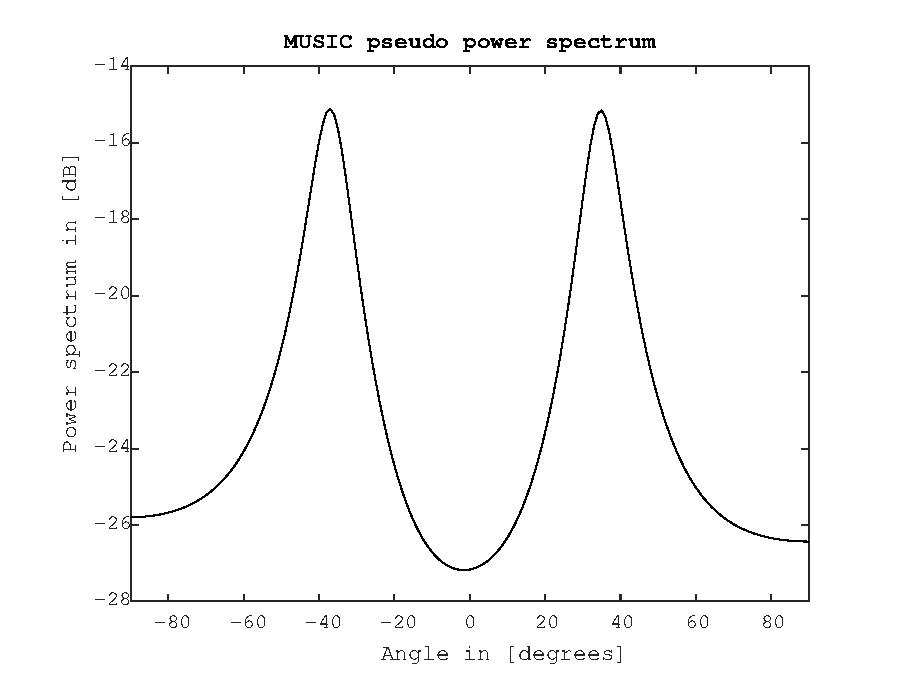
\includegraphics[scale=0.4]{img/after_window.eps}}
\end{figure}

\subsection{Process}
\hspace{0.5em} And we do the experiment with two cotton threads to specify the direction. Two of our members speak at two directions, holding the cotton threads to get precise directions. Using Audacity, we acquired four tracks of sound. Remember to reverse the tracks because of different modeling methods.

\begin{figure}[H]
    \centering
    \subfigure[Test environment]{
        \includegraphics[width=0.4\textwidth]{img/origin.jpg}}
    \hspace{0.4in}
    \subfigure[Output]{
        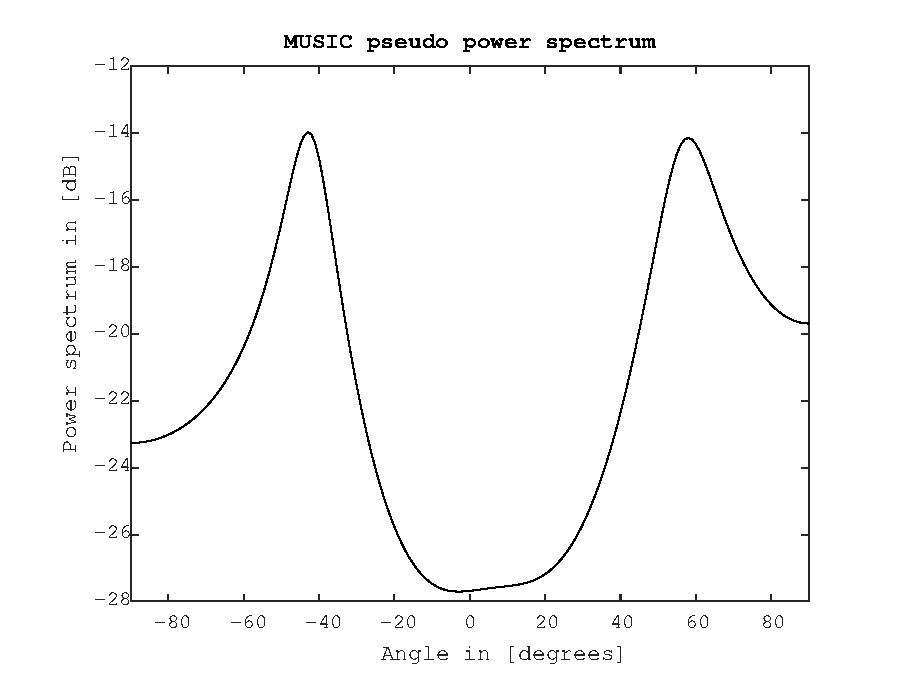
\includegraphics[width=0.4\textwidth]{img/mod3_precise.eps}}
\end{figure}

And the result is rather precise:
\begin{lstlisting}
    The first source with MUSIC is: −43 deg
    The second source with MUSIC is: 58 deg
\end{lstlisting}

\subsection{Real time}
The real time DoA is implemented in \emph{main.m}, and its core is to use \emph{audioDeviceReader()} to get signal from the audio card.

\begin{lstlisting}
devReader = audioDeviceReader( ...
    'Driver', 'DirectSound', ...
    'SamplesPerFrame', fs*samplingTime, ...
    'SampleRate', fs, ...
    'NumChannels', 4, ...
    'BitDepth', '16-bit integer', ...
    'Device', '麦克风 (USB YDB01 Audio Effect)', ...
    'ChannelMappingSource', 'Property', ...
    'ChannelMapping', [2 1 4 3] ...
);
setup(devReader);
\end{lstlisting}
After finishing the initialization, just apply \emph{music} with those segments and display the real-time information.

\subsection{GUI}

\hspace{0.5em} Our GUI finally came out to be:
\begin{figure}[H]
    \centering
    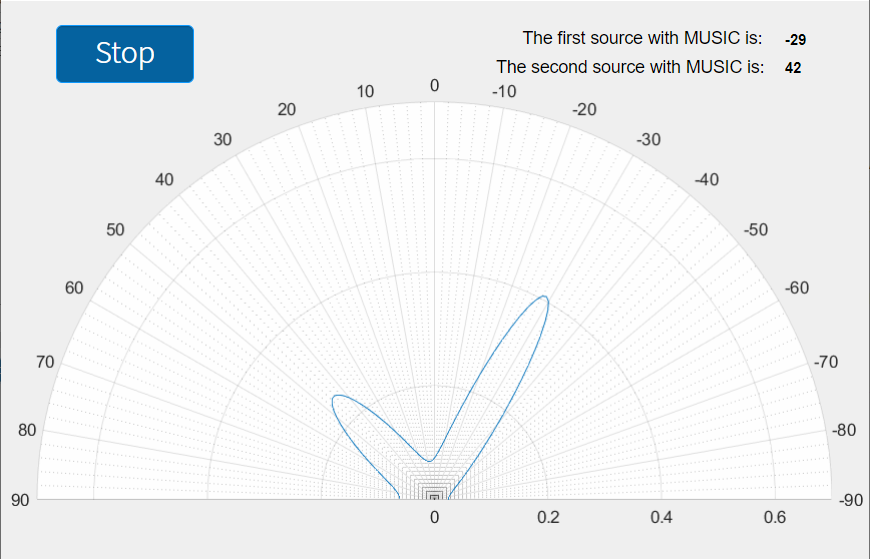
\includegraphics[scale=0.45]{img/GUI.png}
\end{figure}

The GUI part, which focuses on building a user-friendly program doing
the real-time DOA estimation, can show the probability of every
direction of the sound through a polar diagram, and display the most
possible two directions on the interface. The start and stop can be
entirely controlled by a button. It is a task finished with lots of
difficulties and obstacles mostly caused by the unfamiliarity with
MATLAB.

We started with designing an application using MATLAB Guide. But not
long we found that it's really hard to use so we turn to MATLAB App
designer, a more easy-to-use tool. But what we didn't know then was that
it was just the beginning of the tough development process.

Aiming at a GUI which can start and stop the real-time DOA estimation
algorithm at any time, the first thought of us was to conform to the
multi-threaded procedural framework by using the object \emph{timer}
in MATLAB. In fact, it was not only a natural choice but also an
efficient way to control all the program work and stop according to
every "tic" of the \emph{timer}. But soon we found that it caused a
large number of problems, list as follows:

\begin{itemize}
\item
  No graph. Though there're three running modes for \emph{timer}, the
  period is fixed. That means the program itself will pitilessly start
  the next period regardless of the graph has not been plot yet, which
  caused that there will be hard to control the \emph{timer.period} to
  let the graph be plotted.
\item
  Chaos. The timer will never stop unless the \emph{stop} command is
  executed. And if you execute the \emph{start} command while the
  previous \emph{timer} is still running, the command will create
  another \emph{timer} doing the same thing as the previous one, and
  you don't have effective means to tell them apart, which causes that
  all the command become confusing and lead to the total chaos of the
  program.
\item
  Unreasonable bugs. Though the logic of the program is right, the test
  of it discovers many unreasonable bugs, such as unfixed update rate of
  the graph, unexpected crash of MATLAB, not being able to restart after
  stop, etc.
\end{itemize}

So it becomes impossible for us to accomplish the GUI through timer. We
replace it with another construction, which has a prepare part, a main
working part and a stop part. The prepare part does necessary settings
like setup the \emph{audioDeviceReader}, change the text of the
button; the working part do the MUSIC algorithm to estimate the
direction of the sound and update the graph; the stop part help the
program stop properly by release the \emph{audioDeviceReader} and
change the text of the button back. This model works regularly by the
signal produced by the button. Below are the details of how it work.

\begin{enumerate}
\item
  Get started. When the program is first launched, all of the elements
  are set.
\item
  Get prepared. The double-state button is the only controller of the
  whole program. When it turns to "press", which equals its value turn
  to "1", the prepare part is firstly launched by the callback of the
  button.
\item
  Work. Working part runs right after the prepare part. It will continue
  working until the value of the button element comes to "0".
\item
  Stop. When the value of the button element comes to "0", the working
  circulation will be broken and the stop part will do something to
  recover some properties for next time.
\end{enumerate}

Seems really easy, but the problem is, if a callback is working without
special operations, then any other callbacks won't be launched at all.
That means, if the button turns to the other state, its corresponding
callback will just keep pending, and any of the properties of any
elements of the program won't be changed by that. Furthermore, the plot
course will also be interrupted by next working part. It really costs
some time to find out the solution: \emph{drawnow}.

It surely a great breakthrough in finding this suitable function. The
description is "updates figures and processes any pending callbacks".
That means it can plot the graph and change the value of the button to
"0" to let the working part know it should stop next time. However, this
function seems not working every time. It would randomly ignore the
callback caused by the button and continue working without any
hesitation. Till now, we still don't know why \emph{drawnow} sometimes
loses its efficacy, we can only guess that it is caused by the running
mode of MATLAB and its unclear multi-threaded procedural framework. This
surely leaves some regret for the project, but we have really tried our
best.

\begin{thebibliography}{2}
    \bibitem{MUSIC} R. Schmidt, "Multiple emitter location and signal parameter estimation," in IEEE Transactions on Antennas and Propagation, vol. 34, no. 3, pp. 276-280, March 1986, doi: 10.1109/TAP.1986.1143830.
    \bibitem{ISSM} Guaning Su and M. Morf, "The signal subspace approach for multiple wide-band emitter location," in IEEE Transactions on Acoustics, Speech, and Signal Processing, vol. 31, no. 6, pp. 1502-1522, December 1983, doi: 10.1109/TASSP.1983.1164233.
\end{thebibliography}
\end{document}

